\documentclass[5p,times,twocolumn]{elsarticle}

\usepackage{algorithm}
\usepackage[export]{adjustbox}
\usepackage[noend]{algpseudocode}
\usepackage{todonotes}
\usepackage{xspace}
\usepackage{listings}
%\usepackage{subcaption}
\usepackage{paralist}
\usepackage[compact]{titlesec}
\usepackage{balance}
\usepackage{booktabs}
\usepackage{caption}
\usepackage{amssymb,amsmath}
\usepackage[strings]{underscore}

\usepackage{url}
%\usepackage{breakurl}
%\usepackage[hidelinks]{hyperref}
\usepackage{hyperref}
\usepackage[hyphenbreaks]{breakurl}
%\usepackage[hyphens]{url}
\def\UrlBreaks{\do\/\do-}

\newcommand{\mpifunc}[1]{\lstinline"MPI_#1"\xspace}
\newcommand{\prrte}[0]{\textsc{PRRTE}\xspace}
\newcommand{\pmix}[0]{PMIx\xspace}
\newcommand{\orte}[0]{Open~RTE\xspace}
\newcommand{\ompi}[0]{Open~MPI\xspace}
\newcommand{\mpi}[0]{\textsc{MPI}\xspace}
\newcommand{\arm}[0]{Arm\xspace}
\newcommand{\oshmem}[0]{OpenSHMEM\xspace}
\newcommand{\sve}[0]{\textsc{SVE}\xspace}
\newcommand{\armie}[0]{ArmIE\xspace}
\newcommand{\ddt}[0]{\textsc{DDT}\xspace}
\newcommand{\acle}[0]{\textsc{ACLE}\xspace}

\newcommand{\imb}[0]{\textsc{IMB}\xspace}

%\def\BibTeX{{\rm B\kern-.05em{\sc i\kern-.025em b}\kern-.08emT\kern-.1667em\lower.7ex\hbox{E}\kern-.125emX}}

\begin{document}

\title{Using Long Vector Extensions for MPI Reductions}

\author[First]{Dong Zhong\corref{cor1}}
\ead{dzhong@vols.utk.edu}

\author[First]{Qinglei Cao}
\ead{qcao3@vols.utk.edu}

\author[First]{George Bosilca}
\ead{bosilca@icl.utk.edu}

\author[First]{Jack Dongarra}
\ead{dongarra@icl.utk.edu}

\cortext[cor1]{Corresponding author}
\address[First]{The University of Tennessee, 1122 Volunteer Blvd, knoxville, TN 37996}

\begin{abstract}
  %GB: As the scale of high-performance computing (HPC) systems continues to grow, researchers are devoted themselves to explore increasing levels of parallelism to achieve optimal performance.
  % At the ongoing hardware development trend, exploiting all available parallelism on
  % High-Performance Computing (HPC) systems is the only way optimal performance.
  %
  The modern CPU's design, including its features of hierarchical memory and
  SIMD/vectorization capability, governs algorithms' efficiency much more than
  the modest frequency increase we have lately witnessed. The recent
  introduction of wide vector instruction set extensions (AVX and SVE) motivated
  vectorization to become critical software component to increase efficiency and
  close the gap to peak performance.
  %
  % Intel released processor architectures AVX-512 introduced 512-bit extensions to the 256-bit Advanced Vector Extensions instructions for x86 Instruction Set Architecture (ISA). It embraced new capabilities such as flexible memory access, vector mathematical functions, as well as a small set of further instructions for mathematical library support. These new features allow for better compliance with long vector load/store and reduction operations.
  % %
  % ARM's modern Armv8-A architecture also introduced Scalable Vector Extension (SVE) - an optional separate architectural extension with a new set of A64 instruction encodings, which enables even more significant parallelisms.
  %

  In this paper, we investigate the impact of the vectorization of MPI reduction
  operations, and propose an implementation of predefined MPI reduction
  operations using vector intrinsics (AVX and SVE) to improve the
  time-to-solution of the predefined MPI reduction operations.
  %
  The evaluation of the resulting software stack under different scenarios
  demonstrates that the approach is generic and efficient.  Experiments
  conducted on different architectures (Intel Xeon Gold, AMD Zen 2, and Arm
  A64FX), show that the proposed vector extension optimized reduction operations
  significantly reduce completion time for collective communication reductions.
  With these optimizations, we achieve higher memory bandwidth and an increased
  efficiency for local computations, which directly benefit the overall cost of
  collective reductions and applications based on them.
  % than \ompi default for MPI reductions operations.
%
  % Furthermore, we demonstrate the efficiency of our AVX512-enabled approach by
  % a distributed deep learning application Horovod showing 12\% speedup with 1536 processes.
% todo add compare result vs ompi
\end{abstract}

\begin{keyword}
Long vector extension \sep Vector operation \sep Intel AVX2/AVX-512 \sep
Instruction level parallelism \sep Single instruction multiple data \sep
MPI reduction operation \sep Scalable Vector Extension (SVE)
\end{keyword}

\maketitle

\section{Introduction}\label{sec:intro}
The need to satisfy the scientific computing community's increasing
computational demands drives larger HPC systems with more complex architectures,
which provides more opportunities to enhance various parallelism levels.
%
Instruction-level (ILP) and thread-level parallelism (TLP) has been extensively
studied, but data-level parallelism (DLP) is usually underutilized in CPUs, despite its vast potential.
While ILP importance subsides DLP becomes a critical
factor in improving the efficiency of
microprocessors~\cite{energyeffects, HardwareEvents, espasa1998vector, Watson1972TheTA, clusterefficiency}.
The most widespread vector implementation is based on single-instruction multiple-data (SIMD) extensions.
Vector architectures are designed to improve DLP by processing multiple input data simultaneously with a single instruction, usually applied to vector registers.
%or to extract DLP by operating over several input elements with a single instruction.
SIMD instructions have been gradually included in
microprocessors, with each new generation providing more sophisticated, powerful, and flexible
instructions. The higher investment in SIMD resources per core makes extracting
these vector units' full computational power more significant than ever.

A large body of literature has been focusing on employing DLP via vector
execution and code vectorization~\cite{VectorizingCompilers1,vectorizingcompilers,SIMDVectorOperations}, and HPC, with its ever-growing demand for computing capabilities, has been quick to embrace vector processors and harness this additional compute power.
As an essential factor of processors' capability to apply
a single instruction on multiple data, vectorization continuously improves
from one CPU generation to the next by using larger vector registers, gather/scatter capabilities, and much more.
Compared to traditional scalar processors, extension vector processors support
SIMD and more powerful instructions operating
on vectors with multiples elements. They can generate orders of magnitude faster memory accesses and data computations.
%involved rather than a single element, which
%could achieve maximum computational power.
Over the last decade, the difference between a scalar code and its vectorized equivalent
increased from a factor of 4 with SSE, up to a factor of 16 with AVX-512~\cite{PentiumIII,Haswelldetail,avx-info}, highlighting the importance of employing vectorized code whenever possible.
%Therefore, it is essential to vectorize code to achieve high performance on modern CPUs by using dedicated instructions and registers.
The conversion of a scalar code into a vectorized
equivalent can be relatively straightforward for many classes of algorithms
and computational kernels, as it can be done transparently by a compiler
with auto-vectorization. The compiler can provide a baseline for more complex codes,
but developers are also encouraged to offer optimized versions using
widely available compilers intrinsics.
%

There are efforts to improve the vector processors by increasing the vector
length and adding new vector instructions.
As an example, Intel's first version of vectorized instruction set, MMX was quickly superseded by more advanced vector integer SSE and AVX instructions~\cite{intelsse, intelavx, avxsets},
then expanded to Haswell instructions as 256 bits (AVX2),
and then with the arrival of the Knights Landing processor~\cite{avx-info} the more advanced
AVX-512~\cite{Intelref} was introduced supporting 512-bit wide SIMD registers (ZMM0-ZMM31)
as in Figure~\ref{fig:avxmms}. The lower 256-bits of the ZMM registers are
aliased to the respective 256-bit YMM registers, and the lower 128-bit are
aliased to the respective 128-bit XMM registers;
%
%todo rewrite
The AVX-512 features and instructions provide a significant advantage to 512-bit SIMD support.
It offers the highest degree of compiler support by including a unique level of richness
in designing the instructions.
%
Compared to previous architecture and products, it leverages longer and more
powerful registers capable of packing eight double-precision, or sixteen
single-precision floating-point numbers,
or eight 64-bit integers, or sixteen 32-bit integers within a 512-bit vector.
It also enables processing twice the amount of data elements than Intel AVX2 and four
times than SSE with a single instruction.
%
Furthermore,  AVX-512 supports more features such as operations on packed
floating-point data or packed integer data, new operations, additional
gather/scatter support, high-speed math instructions, and the ability to have
optional capabilities beyond the basic instruction set.

\begin{figure}[h]
    \centering
    % trim={<left> <lower> <right> <upper>}
    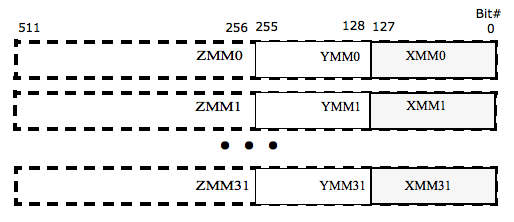
\includegraphics[width=\linewidth]{avx_mms.png}
    \caption{AVX512-Bit Wide Vectors and SIMD Register Set}
    \label{fig:avxmms}
\end{figure}

AVX-512 takes advantage of using long vectors and enables powerful high
vectorization features that can achieve significant speedup. Those features
include but not limited to:
\begin{enumerate}
  %\item using rich addressing mode which enables non-linear data access that can deal with non-contiguous data;
  \item providing a valuable set of horizontal reduction operations which apply to more
  types of reducible loop carried dependencies including both logical, integer
  and floating-point of high-speed math reductions;
  \item and permitting vectorization of loops with more complex loop carried dependencies and more complex control flow.
\end{enumerate}

Similarly, \arm announced the new Armv8 architecture embracing \sve - a vector extension for AArch64
execution mode for the A64 instruction set of the
Armv8 architecture~\cite{arm-v8-ref, ARMv8-Architecture}.
%arm-v8-sve,
Unlike other SIMD architectures, \sve does not define the size of
the vector registers. Instead, it provides a range of different values that permit vector
code to automatically adapt to the current vector length at runtime with the
feature of \emph{Vector Length Agnostic} (VLA) programming~\cite{Advanced-SIMD,vla-stencil}.
Vector length constrains in the range from a minimum of 128 bits up to
a maximum of 2048 bits in increments of 128 bits.

At the other end of the programming spectrum, Message Passing Interface
(\mpi)~\cite{mpi-forum} is a popular, efficient and portable parallel programming
paradigm for distributed memory systems widely used in scientific applications.
The MPI standard provides an entire set of communication primitives, between pairs
of processes or between whole groups of processes,
allowing applications to tailor their use to their needs completely.
%As many scientific applications operate on a large amount of data, manipulating and operating these data become complicated.
%
Therefore, there is no critical subset of MPI capability. In particular, all MPI aspects are
essential to some computation domains.
However, there is evidence that optimized support for two-sided communications and
collective communications will benefit a large number of parallel applications. As an example,
machine learning applications running on distributed systems,
critically depend on the performance of an MPI\_Allreduce, a reduction operation,
for extensive data sets to synchronize updating the weights matrix.

Computation-oriented collective operations such as MPI\_Allreduce and MPI\_Reduce perform reductions on
data along with the communications performed by collectives.
These collectives typically encompass a memory-bound operation, which forces
the computation to become the main bottleneck and limit collective implementation's overall performance.
However, the existence of advanced architecture technologies introduced
with wide vector extension and specialized arithmetic operations, calls for
MPI libraries to provide support for such extensions, providing specialized functions
capable to extracting most of the processor's computational power to deliver it to the application.

%take advantage of advanced vector
%extension (\sve and AVX-512~\cite{avx-info, AVXextensions}).

Unlike more traditional HPC applications that embraced MPI long ago,
machine learning and data science, in general, were more reticent. However,
a new trend has arisen lately, certainly concerning the growth
of the problems' size, toward more extensive use of \mpi for the distributed training.

As mentioned before, the most expensive step in the learning process, the reduction of the gradients, is entirely dependent on the performance of MPI\_Allreduce with a large amount of data (basically all the weights on the layer).
Such reduction operations in machine learning applications
are commonly seen in synchronous parameter updates of the distributed Stochastic
Gradient Descent (SGD) optimization~\cite{sgd10}, which is used extensively
in, for example, neural networks, linear regressions, and logistic
regressions. Usually, this kind of reduction has two aspects: 1) the number of reduction
operations is significant. 2) the data size used by each reduction operation is considerable (with an extensive training model, the data could be in the hundreds of megabytes).
%
Li's~\cite{inproceedings} work explores the performance of allreduce algorithms
and uses task-based frameworks to improve their performance. Specifically talking about AlexNet on ImageNet~\cite{NIPS20124824}, it points out that
each step needs to perform a weights reduction with an estimated size
of 200MB for extensive model training.
%
Similarly, \cite{moritz2015sparknet}
illustrates that with SparkNet, updating the weights of AlexNet, a single reduce
operation takes almost 20 seconds, even on five nodes. While it's relatively simple to scale
the number of execution nodes to the thousands, the biggest bottleneck remains the all reduce of
the gradient values at each step. The size of this reduction is equivalent
to the model size itself, and it is not reduced when more
nodes are used. When scaling to large numbers of nodes, the full parameter set, commonly hundreds of
megabytes, must be summed globally every few microseconds. We can see that, in such cases,
reduction operation dominates the overall time-to-solution in distributed neural network
training, highlighting the need for a more efficient reduction implementation.

Thus, it will be crucial for many applications to provide a highly optimized
version of MPI\_Allreduce, and this requires addressing the challenge of improving the performance of the predefined MPI operations. We tackle the above challenges and provide designs and implementations
for reduction operations, which are most commonly used by the computation
collectives - MPI\_Reduce, MPI\_Allreduce and MPI\_Reduce\_Local.
We propose extensions to multiple \mpi reduction methods to fully take
advantage of the AVX-512 capabilities such as vector product to efficiently
perform these operations.

This paper makes the following contributions:
%\begin{compactenum}
%to do add ML experiments
\begin{enumerate}
  \item We investigate and utilize AVX-512 arithmetic instructions/intrinsics to optimize and
  speed up various \mpi reduction operations.
%
  \item perform experiments using the new reduction operations in the scope
  of \ompi on a cluster supporting the Intel AVX-512 extensions. Different types of
  experiments are conducted with \mpi application, performance evaluation tool, and
  deep learning benchmark.
  %Experiment results demonstrate the efficiency of our AVX-512 optimized reduction
  %operations in \ompi implementation.
  Furthermore, our implementation provides useful insight and guidelines on how vector
  ISA can be used in high-performance computing platforms and software.
      %todo strengthen this is new module in ompi
\end{enumerate}
%\end{compactenum}

The rest of this paper is organized as follows.
%Section~\ref{sec:motivation} motivates our study and provides use cases and
%background on the \sve instructions specific optimization in \mpi implementation in \ompi.
Section~\ref{sec:related} presents related studies on taking advantage of AVX-512 and \sve for specific mathematics applications, together with a survey about optimizations of \mpi to take advantage of novel hardware.
Section~\ref{sec:design} describes the implementation details of our optimized reduction methods in the scope of \ompi using AVX-512 intrinsics and instructions.
Section~\ref{sec:perf} uses a performance too to evaluate performance by different kinds of instruction counts.
Section~\ref{sec:platformsexperiments} displays the extension of reduction work on AMD and Arm platforms.
Section~\ref{sec:hpcapplication} illustrates the performance benefits we achieve by running tests using LAMMPS benchmark.
Section~\ref{sec:experiments} describes the performance difference between
\ompi and AVX-512 optimized \ompi and provides a distinct insight on how the
new vector instructions can benefit \mpi.
Section~\ref{sec:application} illustrates our optimized reduction operation's performance
benefits in \ompi using a deep learning application.

\section{Related Work}\label{sec:related}
Different techniques can be roughly classified according to the level at which
the hardware supports parallelism with multi-core and multi-processor computers having
multiple processing elements within a single machine. Different level of parallelization,
including bit-level, instruction-level, data-level, and task parallelism, are studied.
%
In this section, we survey related work on techniques taking advantage of
advanced hardware or architectures, which mainly focuses on data-level parallelization.
Novel processors and hardware architectures from different vendors, such as Intel and Arm,
come equipped with long vector extensions, and multiple researchers have studied the usage
of those new technologies in high-performance computing with various programming models and applications.
%
\subsection{Long vector extension}
Lim~\cite{Lim2018} explored matrix-matrix multiplication based on blocked matrix multiplication
improves data reuse. They used data prefetching, loop unrolling, and the Intel AVX-512
to optimize the blocked matrix multiplications, which achieved outstanding performance of GEMM
with single and multiple cores.
%
Kim~\cite{Kim19} presented an optimal implementation of single-precision and double-precision general matrix-matrix multiplication (GEMM) routines based on an auto-tuning approach with the Intel AVX-512 intrinsic functions.
The implementation significantly reduced the search space and derived optimal parameter sets, including the size of submatrices, prefetch distances, loop unrolling depth, and parallelization scheme.
%
Bramas~\cite{Bramas2017} introduced a novel quicksort algorithm with a new Bitonic sort and a new
partition algorithm that has been designed for the AVX-512
instruction set, which showed superior performance on Intel SKL in
all configurations against two standard reference libraries.
%
A little closer to MPI, Dosanjh et al.~\cite{tag-match} proposed and evaluated a novel message matching method Fuzzy-matching
to improve the point to point communication performance in MPI with multithreading enabled.
The proposed algorithm took advantage of the AVX vector operation to accelerate matches
and demonstrated that the benefits of vector operation are not only restricted to computational intensive operations, but can positively impact MPI matching engines. They also presented an optimistic
matching scheme that uses partial truth in matching elements
to accelerate matches.
%
Intel AVX is not the only ISA to propose vectorized extensions. Similar studies have been done using Arm's new scalable vector SVE.
In this work~\cite{sve-stencil}, they leveraged the characteristics of \sve to implement and optimize
stencil computations, ubiquitous in scientific computing which showed
that \sve enabled the easy deployment of optimizations like loop unrolling,
loop fusion, load trading or data reuse.
%
Petrogalli's work~\cite{sveml} explored the usage of SVE vector multiple
instructions to optimize matrix multiplication in machine learning algorithm.
%
Zhong~\cite{dongsve} used SVE load, gather and scatter instructions to optimize MPI datatype
packing and unpacking in \ompi.
%
We can see those work focused on using new instructions to improve a specific application's performance or a specific mathematical algorithm.
In our work, we study AVX-512 enabled features more comprehensively for
all supported mathematical reduction functions and also provide
a detailed analysis of the efficiency achievements of related intrinsics.
Furthermore, we aim to accommodate the AVX reduction instructions support in MPI to provide
vectorized computations for applications.

\subsection{\mpi reduction operation}
Additionally, different techniques and
efforts have been studied to optimize \mpi reduction operations. Traff
~\cite{NeutralMPIReduction} proposed a simple implementation of MPI library
internal functionality that enabled MPI reduction operations to be performed
more efficiently with increasing input vectors' sparsity.
%
Also Chu~\cite{gpu-reduce} analyzed the limitations of the compute oriented CUDA-Aware
collectives and proposed alternative designs and schemes by combining the exploitation GPU's
compute capability and their fast communication
path using GPUDirect RDMA feature to alleviate these limitations efficiently.
%
Luo~\cite{Luo-adapt} presented a collective communication framework called ADAPT
in \ompi based on an event-driven infrastructure. Through events and callbacks,
ADAPT relaxed synchronization dependencies and maintained the minimal data dependencies.
This approach provided more tolerance to system noise and also supported fine-grained,
multi-level topology-aware collective operations, which can exploit the
parallelism of heterogeneous architectures.
%
Hofmann~\cite{sparse-reduction} presented a pipeline algorithm for MPI Reduce
that used a Run Length Encoding scheme to improve the global reduction of sparse
floating-point data.
Patarasuk's work~\cite{allreduce-optimal} investigated implementations of the allreduce operation
with large data sizes and derived a theoretical lower bound on this operation's communication time and developed
a bandwidth optimal allreduce algorithm on tree topologies.
%
Shan~\cite{shan-reduce} proposed using idle threads on a many-core node to accelerate
the local reduction computations and utilized the data compression technique to compress sparse input data for reduction.
Both approaches (threading and exploitation
of sparsity) helped accelerate MPI reductions on large vectors when
running on many-core supercomputers.
%

Most of those work focuses on improving the performance of
communication either by relaxing dependencies or hiding the communication latency behind computation.
And for the minority of those work that endeavors to strengthen the computation part,
they usually have some requirements or limitations of data
representation or need extra hardware such as GPUs.
Our long vector extension arithmetic reduction
optimizations seek to be more general and use the newly available vector extensions to provide a
straightforward set of predefined MPI operations, with no data representation or operations limitation.
The implementation supports multiple ISA (x86 and AArch64), covering most processor versions from different vendors,
which support legacy SSE, advanced AVXs, and SVE.

\section{Design and implementation}\label{sec:design}
\subsection{Intel Advanced Vector Extension}
Intel Advanced Vector Extension 2 (Intel AVX2), is a significant improvement to Intel Architecture.
It supports the vast majority of previous generations 128-bit SIMD float-point
and integer instructions to operate on 256-bit YMM registers to support 256-bit operations.
%
AVX2 also enhances a vibrant mix of broadcast, permute/variable-shift instructions to accelerate
numerical computations. The Intel microarchitecture Haswell supports the 256-bit AVX2 instructions
implementing 256-bit data path with low latency and high throughput.
Besides, AVX2 provides enhanced functionalities for broadcast and permute operations on data elements,
vector shift instructions with variable-shift count per data element,
and instructions to fetch non-contiguous data elements from memory.

Moreover, Intel Advanced Vector Extensions 512 (Intel AVX-512) instructions
enrich significant supports compared to AVX2. It provides more powerful packing
capabilities with longer vector length, such as encapsulating eight double-precision
or sixteen single-precision floating-point numbers,
or eight 64-bit integers, or sixteen 32-bit integers within a vector.
The longer vector enables processing twice the number of data elements
than that of Intel AVX/Intel AVX2 can
process with a single instruction and four times than that of SSE.
On the other hand, it contributes to more outstanding performance for the most
demanding computational tasks with more vectors(32 vector registers, each 512 bits wide,
eight dedicated mask registers), enhanced high-speed math instructions, embedded rounding controls,
and compact representation of large displacement value.

Furthermore, Intel AVX-512 instructions offer the highest degree of compiler
support by including an unprecedented level of richness in the design of the instructions.
Thus, it has better compatibility with Intel AVX that is stronger than
prior transitions to new widths for SIMD operations.
For SSE and AVX, programs will suffer from performance penalties once mix them.
However, the mixing of AVX and Intel AVX-512 instructions is supported without penalty.
AVX registers YMM0--YMM15 map into the Intel AVX-512 registers
ZMM0--ZMM15, very much like SSE registers map into AVX registers. Therefore, in processors with
Intel AVX-512 support, AVX and AVX2 instructions operate on the lower 128 or 256 bits of the first 16 ZMM registers.

\subsection{Intrinsics}
Intel intrinsics are built-in functions that provide access to the ISA functionality
using C/C++ style coding instead of assembly language. Without Intel intrinsic was
supported, users had to write assembly code directly to manipulate SIMD
instructions arbitrarily.
However, Intel has defined several sets of intrinsic functions that are implemented
in the Intel Compiler. These types empower the programmer to directly choose the implementation
of an algorithm while allowing the compiler to perform register allocation
and instruction scheduling wherever possible. The intrinsics are portable among all
Intel architecture-based processors supported by a compiler. The use of intrinsic
allows developers to obtain performance close to the levels achievable and feasible with assembly.
The cost of writing and maintaining programs with intrinsics is considerably less than writing assembly code.
In summary, the intrinsic function allows SIMD instructions to be manipulated faster, more
accurately, and more effectively than writing lower-level code.
We describe the primary AVX-512 intrinsic functions that we are interested in our kernel:

\begin{enumerate}[]%[leftmargin=*]
  %
  \item \emph{\textbf{\textit{\_\_m512i\ \_mm512\_loadu\_si512\ (void const* mem\_addr)}}} \\
  Load 512-bits of integer data from memory into a register. The mem\_addr does not need to be aligned on any particular boundary.
  Generally, this instrinsic is converted into:\\
  \emph{\textbf{\textit{vmovdqu32  zmm,  m512}}}.
  %
  \item \emph{\textbf{\textit{\_\_m512i\ \_mm512\_ $\langle op \rangle$ \_epi32\ (\_\_m512i a,\ \_\_m512i b)}}}
  Apply $\langle op \rangle$ between packed 32-bit integers in "a" and "b", and store the results in destination, here we use 32-bits integer as an example.
  Generally, this instrinsic is converted into:\\
  \emph{\textbf{\textit{vp $\langle op \rangle$  m512,  m512,  m512}}}.
  %
  \item \emph{\textbf{\textit{\_\_m512i\ \_mm512\_storeu\_si512\ (void const* mem\_addr,\\ \_\_m512i a)}}}
  Store 512-bits of integer data from "a" into memory. mem\_addr does not need to be aligned on any particular boundary.
  Generally, this instrinsic is converted into:\\
  \emph{\textbf{\textit{vmovdqu32  m512, zmm}}}.
  %
\end{enumerate}

\subsection{Reduction operation in \ompi}
We implement our advanced reduction operation with AVX, AVX2, AVX-512
support in a component in \ompi, based on a Modular Component
Architecture~\cite{dongprrte} that facilitates extending or
substituting \ompi core subsystem with new features and innovations.
We add our long vector reduction optimization in a specialized component that
implements all predefined MPI reduction operations with vector
reduction instructions, as in Figure~\ref{fig:avxmca}. From a
practical standpoint, our module will extract the processor
feature flag and check related flags, selecting at runtime the set of
functions supporting the most advanced ISA (AVX-512, AVX2 or AVX/SSE),
or fallback to the default basic module if the processor has no
support for such extensions, as shown in Figure~\ref{fig:512flow}.
%
To be more specific, we explicitly check CPUID -- a processor
supplementary instruction allowing software to discover the
processor details, determine processor type, and whether features such as
SSE/AVXs are implemented and supported.

\begin{figure}[h]
    \centering
    % trim={<left> <lower> <right> <upper>}
    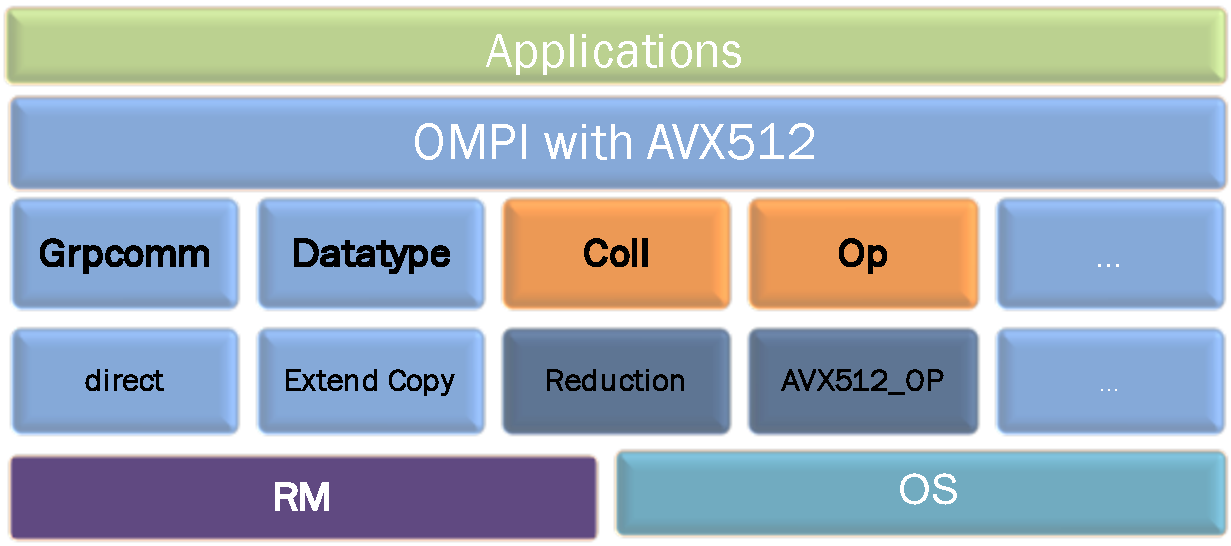
\includegraphics[width=\linewidth]{avx-mca.pdf}
    \caption{\ompi architecture. The orange boxes represent components with added AVX-512 reduction features. The dark blue colored boxes are new modules.}
    \label{fig:avxmca}
\end{figure}

\begin{figure}[h]
    \centering
    % trim={<left> <lower> <right> <upper>}
    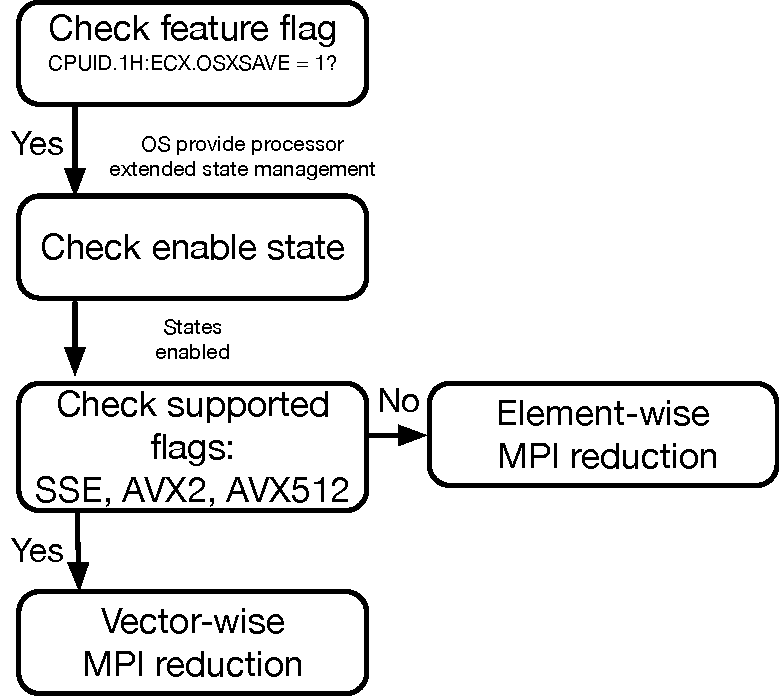
\includegraphics[scale=.45]{avx-graph.pdf}
    \caption{Integrate and automatically activate the AVX component into the \ompi build system}
    \label{fig:512flow}
\end{figure}

To be noted, the computational benefit in our component and modules can be
extended out the scope of reduction operation to general mathematics and logic operations.
This advanced operation module/code-snippet can be easily adapted to other computational intensive software stacks.

To use vector instructions in applications, it can be exploited in several fashions:
(a) relying on automatic vectorization support provided by the compiler;
(b) explicitly calling vector instructions from assembly or via intrinsic functions;
(c) adapting intrinsic functions into programming models or languages
for applications to use.
%
The first strategy by using auto-vectorization, is portable and
"future-proof", which means that it can quickly adapt code to a future
generation of processors, with the only required step being a
re-compilation of the code. However, to effectively use automatic
vectorization, programmers must follow guidelines and restrictions for
vectorizable code and provide compile-time options largely dependent
on a specific compiler's capability and efficiency.
%
And programmers also need to be aware of the specifics of the
instructions that are supported by a processor.  Additionally,
compilers have substantial limitations in the analysis and code
transformations phases that prevent an efficient extraction of SIMD
parallelism in real applications~\cite{autoEvaluation}.
%
The second method allows more control over the very low-level
instruction stream, but the use of intrinsics is time-consuming and
error-prone for application programmers and users.
%
For our work, to integrate the use of AVX-512 features in the \ompi
stack, we prefer to adopt the second approach -- we use intrinsics and
compile flags together to guide the compiler in the vectorization
phase to maximize performance.

\begin{algorithm}[!ht]
\caption{AVX based reduction algorithm}\label{fig:reducealgorithm}

\textbf{\textit{types\_per\_step}} \Comment{Number of elements in vector}\\
\textbf{\textit{left\_over}} \Comment{Number of elements waiting for reduction}\\
\textbf{\textit{count}} \Comment{Total number of elements for reduction operation}\\
\textbf{\textit{in\_buf}} \Comment{Input buffer for reduction operation}\\
\textbf{\textit{inout\_buf}} \Comment{Input and output buffer for reduction operation}\\
\textbf{\textit{sizeof\_type}} \Comment{Number of bytes of the type of the in\_buf / inout\_buf}\\

\begin{algorithmic}[1]
\Procedure{ReductionOp}{ $in\_buf, inout\_buf, count$ }
%\If {( $blocklen$ $\geqslant$ $svcntb$ )}
  \State $types\_per\_step$ = $vector\_length (512)$ / ($8$ $\times$ $sizeof\_type$)
  % \EndIf
  \State{\#pragma unroll}
\For { $k \gets types\_per\_step $ to $ count$}
  \State {\_mm512\_loadu\_si512 from $in\_buf$}
  \State {\_mm512\_loadu\_si512 from $inout\_buf$}
  \State {\_mm512\_reduction\_op}
  \State {\_mm512\_storeu\_si512 to $inout\_buf$}
  \State {Update left\_over}
\EndFor
\If {( $left\_over$ $\neq$ $0$ )}
  \State Update $types\_per\_step >>= 1$
    \If {( $types\_per\_step$ $\leq$ $left\_over$)}
    \State {\_mm256\_loadu\_si256 from $in\_buf$}
    \State {\_mm256\_loadu\_si256 from $inout\_buf$}
    \State {\_mm256\_reduction\_op}
    \State {\_mm256\_storeu\_si256 to $inout\_buf$}
    \State {Update left\_over}
    \EndIf
\EndIf
\If {( $left\_over$ $\neq$ $0$ )}
  \State Update $types\_per\_step >>= 1$
    \If {( $types\_per\_step$ $\leq$ $left\_over$)}
    \State {\_mm\_llddqu\_si128 from $in\_buf$}
    \State {\_mm\_llddqu\_si128 from $inout\_buf$}
    \State {\_mm128\_reduction\_op}
    \State {\_mm\_storeu\_si128 to $inout\_buf$}
    \State {Update left\_over}
    \EndIf
\EndIf
\If {($ left\_over$ $\neq$ $0$ )}
%\tcp*{Duff's device}
  \While{( $left\_over$ $\neq$ $0$ )}{
    \State {Set case\_value}
    \State {\textbf{Switch}(case\_value) : \{8 Cases\}}
    \State {Update left\_over}
  \EndWhile
  }
\EndIf
\EndProcedure
\end{algorithmic}
\end{algorithm}

A reduction is a typical operation encountered in many scientific applications.
Those applications have large amounts of data-level parallelism and should be able
to benefit from SIMD support for reduction operation. Especially in deep learning applications,
it needs to frequently calculate and update the gradients, which is typically very computation extensive.
Traditional reduction operation performs element by element of the input buffers,
which executes as a sequential operation or possible could be vectorized
under particular circumstance or with a specific compiler or constraints. Sometimes
it may suffer from dependencies across multiple loop iterations.
%
Figure~\ref{fig:sseavx} illustrates the difference between a scalar operation and
a vector operation for AVX, AVX2 or AVX-512, respectively.
%
It is an example of a vector instruction processing multiple elements together at the same time,
compared to executing the additions sequentially. A scalar processor would have to perform one load,
one computation, and one store instruction for every element. A vector processor performs one load,
one computation, and one store for multiple elements.
An AVX-512 SIMD-vector can process multiple elements at
the same time. For example, it can store eight double-precision floating-point numbers or 16 integer values, also allow the computation of those elements by executing a single instruction.
AVX-512 reduction instructions perform arithmetic horizontally across active elements of a
single source vector and deliver a scalar result.

\begin{figure}[h]
    \centering
    % trim={<left> <lower> <right> <upper>}
    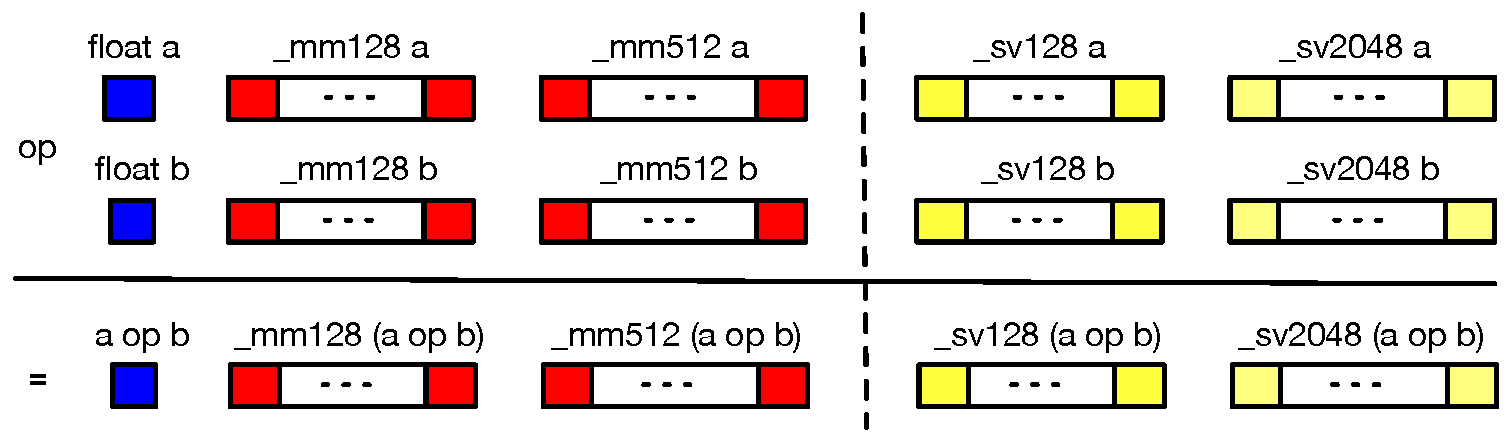
\includegraphics[width=\linewidth]{sse_avx.pdf}
    \caption{Example of single precision floating-point values using : (\colorbox{blue}{}) scalar standard C code, (\colorbox{green}{}) AVX SIMD vector of 4 values , (\colorbox{red}{}) AVX2 SIMD vector of 8 values, (\colorbox{yellow}{}) AVX-512 SIMD vector of 16 values}
    \label{fig:sseavx}
\end{figure}

Intel AVX-512 intrinsic provides arithmetic reduction operation for integer and
float-pointing, also supports logical reduction operations for an integer type.
This gives the chance to create AVX-512 intrinsic-based reduction support in \mpi which
will highly increase \mpi local reduction's performance.
Additionally, AVX-512 can perform scatter reduction operation with the
support of predicate register, which behaves in a vectorized manner. This profoundly
expands the limitation of consecutive memory layout for reduction operation to non-contiguous
data sets at the same time generic and efficient, but such operations
are not needed for the predefined MPI reduction operations.

%
For our optimized reduction operation, we employ and apply multiple
methods to investigate how to achieve the
best performance on different processors, as shown in algorithm\ref{fig:reducealgorithm}.
For a better description, in the rest of the paper, we assume that the hardware supports AVX-512.
%avx512
In the algorithm's for-loop section: First of all, we explicitly use 512 bits long vector loads and stores for memory operation rather than using the memory copy (memcpy) function provided by
the standard library, because some systems and compilers may not perform
the best assembling techniques of using ZMM registers to load and store.
%
After we have the elements loaded in registers, we apply mathematical vector operation
to perform a reduction on the whole vector.
%avx2
We repeat this pattern until the remainders cannot fulfill a 512 bits vector,
then we fallback to use YMM registers to process elements that fit in the 256 bits registers.
And so on, then we execute with 128 bits vectors.
%Duff

Eventually, we reach the last section of the optimization. We have
noticed that depending on the number of elements to apply the
operation on, significant execution time is often spent in the
prologue, that deals with the remainder, those few elements that cannot fulfill a vector.
Intel provides AVX mask intrinsics for mask operations that can vectorize the remainder loop.
Still, significant overhead is involved in creating and initializing the mask and
executing a separate and additional code path, which can result in low SIMD efficiency.
%
The vectorized remainder loops can be even slower than the scalar executions,
because of the overhead of masked operations and hardware.
%
Typically the compiler can determine if the remainder should be vectorized
based on an estimate of the potential performance benefit. When trip count information for a
loop is unavailable, however, it will be difficult for the
compiler to make the right decision.
%
Therefore, for the remainder, we use Duff's
device~\cite{wiki:duff} manually implementing a loop unrolling by
interleaving two syntactic constructs of C: the do-while loop and a
switch statement, which helps the compiler to optimize the device
correctly.
%
We benefit from two aspects of Duff's device. First of all, the loop is unrolled,
which trades larger code size for more speedup by avoiding some of the overhead
involved in checking whether the loop is finished or jump back to the
top of the loop.
It can run faster when it is executing straight-line code instead of jumping.
The second aspect is the switch statement. It allows the code to jump into the middle of the
loop the first time through.
Execution starts at the calculated case label, and then it falls through to each successive
assignment statement, just like any other switch statement.
%
After the last case label, execution reaches the bottom of the loop, at which point it jumps back to the top. The top of the loop is inside the switch statement, so the switch is not re-evaluated anymore.
%
Our Duff's device loop uses eight cases in the switch statement, so the number of iterations is divided by eight.
If the remaining elements to be processed aren't multiple of eight, then some elements are left over.
Most algorithms first deal with blocks of 8 elements at a time and then handle the remainders (less than eight) at the end,
but our Duff's device code processes the remainders (less than eight) at the beginning.
The function calculates "count \% 8" for the switch statement to figure out what the remainder will be, and jumps to the case label for that many elements.
Then the loop continues to deal with blocks of eight elements.

%
Table~\ref{tab:parameters} shows the variety of \mpifunc{Types} and
\mpifunc{Ops} are supported in our optimized reduction operation
module, which matches the combination of types and operations defined
by the \mpi standard.
% We can see our implementation supports all combination of all types
% and operations in \mpi standard.  "-" indicates the logistic
% operations that are not applicable for float pointing.
Table\ref{tab:parameters1} lists the supported x86 instruction set
architectures and related CPU flags from legacy SSE to the latest
AVX-512 instruction sets, together with the corresponding
\emph{\textbf{\textit{op_avx_support}}} values that can be used to select
which AVXs to use if they are supported by the hardware.
To be noted, our work mainly focuses on the
"Fundamental" feature instruction set with flag AVX512F, available on
Knights Landing processors and Intel Xeon processors. It contains
vectorized arithmetic operations, comparisons, type conversions, data
movement, data permutation, bitwise logical operations on vectors and
masks, and miscellaneous math functions. This is similar to the core
feature set of the AVX2 instruction set, with the difference of more
comprehensive and more extended registers, and more functional supports for
float-pointing and integer.

\begin{table}
  \centering
  \caption{Supported types and operations}\label{fig:notations}
  \label{tab:parameters}
  \small
  \begin{tabular}{cclll}
    \toprule
    \texttt{\bf Types} & uint8 - uint64 & float & double \\
    \midrule
    \texttt{\bf MAX} & \checkmark & \checkmark & \checkmark \\
      \texttt{\bf MIN} & \checkmark & \checkmark & \checkmark \\
      \texttt{\bf SUM} & \checkmark & \checkmark & \checkmark \\
      \texttt{\bf PROD} & \checkmark & \checkmark & \checkmark \\
      \texttt{\bf BOR} & \checkmark & --- & --- \\
      \texttt{\bf BAND} & \checkmark & --- & --- \\
      \texttt{\bf BXOR} & \checkmark & --- & --- \\
      \bottomrule
  \end{tabular}
\end{table}

\begin{table}
  \centering
  \caption{Supported CPU flags}\label{fig:cpuflags}
  \label{tab:parameters1}
  \small
  \begin{tabular}{cclll}
    \toprule
    \texttt{\bf Instruction Sets} & CPU flags and & \\ & op_avx_support value & \\
    \midrule
    \texttt{\bf AVXs} & AVX512BW (0x200) & AVX512F (0x100) \\ & AVX2  (0x020) & AVX   (0x010) \\ \\
      \texttt{\bf SSE} & SSE4 (0x08) & SSE3 (0x04) \\ & SSE2 (0x02) & SSE (0x01) \\
      \bottomrule
  \end{tabular}
\end{table}

\section{Performance tool evaluation}\label{sec:perf}
%/todo fix text
To understand the performance, we analyzed our AVX-512 enabled \ompi reduction
operation using Performance API (PAPI)~\cite{papi} -- a tool that can expose
hardware counters, allowing developers to correlate these counters
with the application performance.
% in these increasingly complex environments, and must also
% increase the richness of their measurements to provide insights into the
% increasingly intricate ways in which software and hardware interact.
PAPI is a portable and efficient API to access hardware performance
monitoring registers/counters found on most modern microprocessors.
%It is also a standard API for accessing hardware
%performance counters available on most modern microprocessors.
These counters exist
as a small set of registers that count "events", which are occurrences of specific signals
and states related to the processor's function. Monitoring these events facilitates
correlation between the structure of source or object code and the efficiency of the mapping
of that code to the underlying architecture. This correlation has a variety of uses in
performance analysis and tuning.

%a standard application programming interface (API) for accessing
%hardware performance counters available on most modern microprocessors. These counters exist as a small set of
%registers that count events, which are occurrences of specific signals related to the processor’s function.

We aim to use hardware performance counters in PAPI to measure two aspects:
(1) Memory operation instructions: the total number of load and store instructions.
(2) Branching instructions: number of branch execution instructions including branch instructions taken and not-taken,
instructions mispredicted and instructions correctly predicted, which have a significant impact on performance.
For example, mispredicted branches can disrupt streams of micro-ops or cause
the execution engine to waste execution resources on executing
streams of micro-ops in the non-architected code path.

\begin{figure}[h]
    \centering
    % trim={<left> <lower> <right> <upper>}
    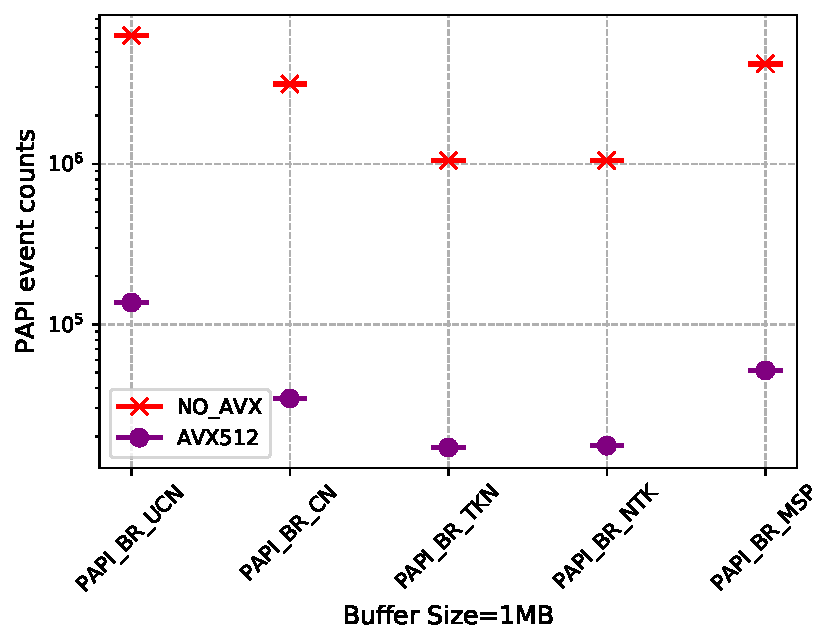
\includegraphics[width=\linewidth]{papi_ins_review.pdf}
    \caption{Comparison between AVX-512 optimized OMPI and default OMPI for MPI\_SUM reduction with PAPI instruction events overview}
    \label{fig:papiins}%\vspace{-0.3cm}
\end{figure}

\begin{figure}[h]
    \centering
    % trim={<left> <lower> <right> <upper>}
    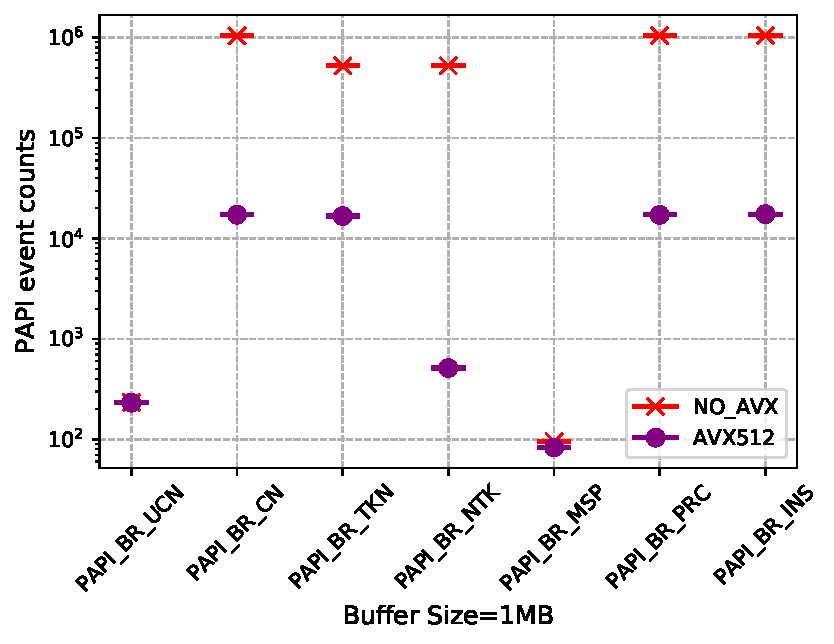
\includegraphics[width=\linewidth]{papi_BR_review.pdf}
    \caption{Comparison between AVX-512 optimized OMPI and default OMPI for MPI\_SUM reduction with PAPI branch counters}
    \label{fig:papibr}
\end{figure}

Figure~\ref{fig:papiins} shows the total number of instructions, and memory access instructions of
load and store, and branch instructions (due to the
stability of the results we choose not to clutter the graphs with
standard deviation).
We can see that for our optimized reduction operation, the total number of
instructions is largely reduced. Also, memory access and branch instructions
have decreased compared to the default implementation in \ompi.
%to do add more
The explanation here is straightforward: longer vectors can load and store more
elements with each instruction than non-vector loads and stores, which means that
we need fewer loads and stores dealing with the same amount of reduction data.
Consequently, this will decrease the loop iteration.
%
Our implementation reduced the number of loads and stores instructions
by a factor of 90X and 60X, respectively.  At the same time, for
branching instructions, our optimization decreased by 60X.  We also
investigated the cache misses of L1 and L2 caches. Because we are
dealing with extensive contiguous data, which means data access
patterns are very regular and easy to predict. All predicted accesses
would be consumed so that the cache misses do not show significant
variation.

Figure~\ref{fig:papibr} illustrates the instruction count details
of branch instructions of both AVX-512 optimized implementation and the default
element-wise reduction method. By using long vectors, we largely decreased the "for loop" of the reduction
operation. Consequently, the AVX-512 code has much less control and branching instructions.
Which means we have less conditional branch instructions.
For conditional branch instructions not taken, we gain
more benefits compared to others, which shows conditional branch instructions are being correctly predicted.
%todo add more with description

%PAPI_BR_UCN  0x8000002a  Yes  Unconditional branch instructions
%PAPI_BR_CN   0x8000002b  No   Conditional branch instructions
%PAPI_BR_TKN  0x8000002c  Yes  Conditional branch instructions taken
%PAPI_BR_NTK  0x8000002d  No   Conditional branch instructions not taken
%PAPI_BR_MSP  0x8000002e  No   Conditional branch instructions mispredicted
%PAPI_BR_PRC  0x8000002f  Yes  Conditional branch instructions correctly predicted
%PAPI_BR_INS  0x80000037  No   Branch instructions
%PAPI_TOT_INS 0x80000032  No   Instructions completed
%PAPI_LD_INS  0x80000035  No   Load instructions
%PAPI_SR_INS  0x80000036  No   Store instructions
%PAPI_LST_INS 0x8000003c  Yes  Load/store instructions completed

\section{Experimental evaluation}\label{sec:experiments}
We conduct our experiments on a local cluster which is an Intel(R)
Xeon(R) Gold 6254 (AVX512F) based server running at 3.10 GHz. Our work is based
upon \ompi master branch, revision \#75a539. Each experiment is
repeated 30 times, and we present the average results.
%(due to the
%stability of the results we choose not to clutter the graphs with
%standard deviation).
We use a single node with one
process for all tests, because our optimization aims to improve the performance of
the computation part of reduction operation rather than the
communication.

This section compares the performance of the reduction operation with two
implementations.
For \ompi default reduction operation base module, it
performs element-wise computation across two input buffers. For each loop iteration,
it processes two elements. Our new implementation uses AVX-512 vector instruction
executing reduction operation on the same inputs, but for each iteration, it
deals with two vectors containing all the elements within the vectors which represent
a vector-wise operation.
For the reduction benchmark, we use the \mpifunc{Reduce_local} function call to
perform the local reduction for all supported MPI operations utilizing an array of different sizes.

We present to compare arithmetic SUM and logical BAND with reduction data size from 1KB to 128MB.
For the experiments, we flushed cache to ensure we are not reusing cache for a fair comparison.

\begin{figure}[h]
    \centering
    % trim={<left> <lower> <right> <upper>}
    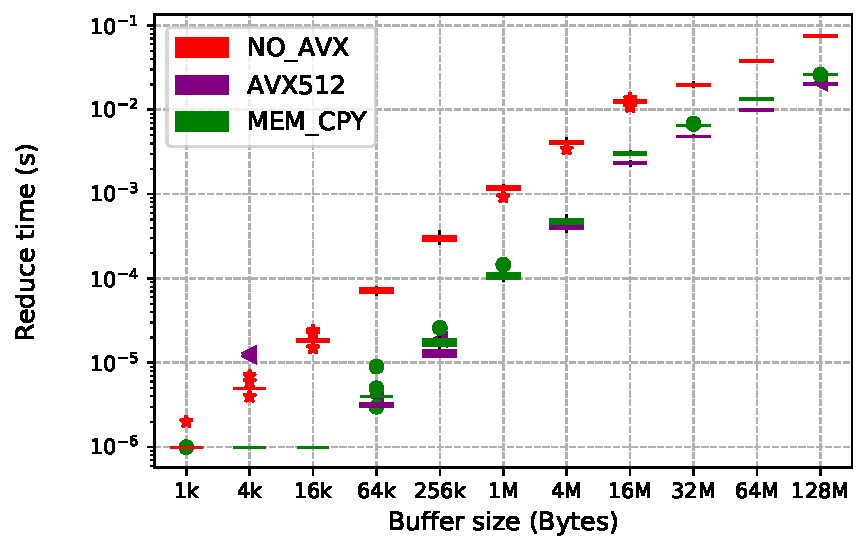
\includegraphics[width=\linewidth]{avx_extend_more_sum_u8_1k-128M.pdf}
    \caption{Comparison of MPI\_SUM with AVX-512 reduction enable and disable for MPI\_UINT8\_T together with memcpy}
    \label{fig:avxsum}
\end{figure}

\begin{figure}[h]
    \centering
    % trim={<left> <lower> <right> <upper>}
    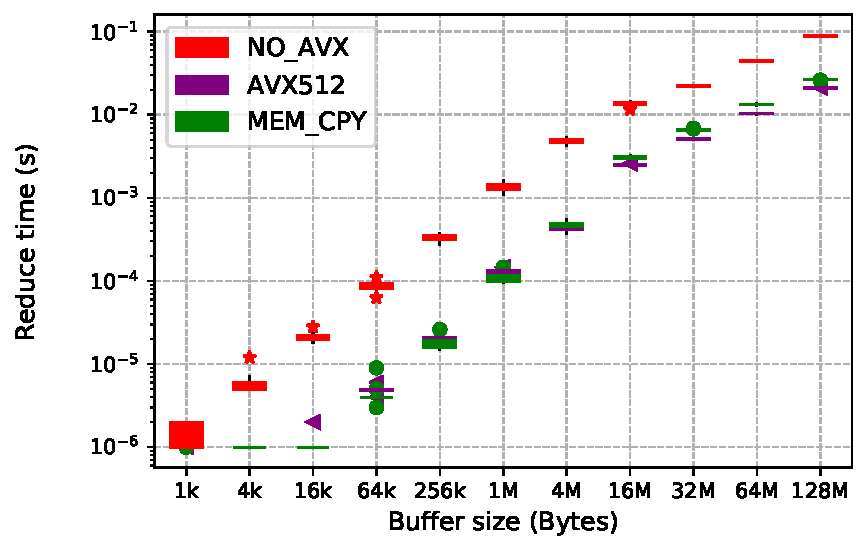
\includegraphics[width=\linewidth]{avx_extend_more_prod_u8_1k-128M.pdf}
    \caption{Comparison of MPI\_BAND with AVX-512 reduction enable and disable for MPI\_UINT8\_T together with memcpy}
    \label{fig:avxband}
\end{figure}

Figure~\ref{fig:avxsum} and Figure~\ref{fig:avxband} show the result for the
\mpifunc{SUM} and \mpifunc{BAND}.
%, due to the limited length of the paper, we cannot
%include the assemble code here.
It should be noted for the default \ompi's compiler, despite the
provided optimization flags, did not generate auto-vectorized
code. Our optimization uses intrinsics which gives us complete
control of the low-level details at the expense of productivity and
portability.

Results demonstrate that using AVX-512 enabled operation the
performance can be improved by order of magnitude compared with the
element-wise operation.  To be more specific, when the total size of
the reduction elements is small, the performance benefit remains low.
%
However, when the buffer size bigger than 4KB, the performance
advantage becomes considerable and stable.  We also compare MPI
operation and memory copy, which indicate the peak memory bandwidth
for a similar operation.  To make a fair comparison, we list the
complete execution sequence of reduction operation and memory copy
operation.  We can see that for a \mpi reduction operation, it needs
two loads from both input memory, and then an additional
computation, eventually followed by one store to save the results into
memory. For memcpy it only needs one load from source and one store to
destination.  The result shows that even with an additional
computation included, our optimized AVX-512 reduction operation
achieves a high level of memory bandwidth comparable to
memory copy.  To be remarked, when the reduction buffer size increases,
our implementation achieves the same performance as
memory copy, which indicates we maximize the memory bandwidth.

\section{Experimental evaluation with different platforms}\label{sec:platformsexperiments}
\subsection{AMD Zen 2 architecture}
AMD's new Zen architecture supports all the latest x86 instructions such as SSE and AVX/2.
But the data paths are 128 bits wide, the way 256-bit AVX was designed but be carried
out as two independent 128-bit operations.
It needs split up 256-bit operations into two 128-bit operations, which means 256-bit operations will
use up twice the resources to complete. Thus, the peak throughput is four SSE/AVX-128 instructions or two AVX-256 instructions per cycle.

The Zen 2 architecture doubles the physical registers' width, execution units, and data paths to 256 bits.
This improvement doubles the peak throughput of AVX-256 instructions to four per cycle, or in other words,
up to 32 FLOPs/cycle in single precision or up to 16 FLOPs/cycle in double precision.

\begin{figure}[h]
    \centering
    % trim={<left> <lower> <right> <upper>}
    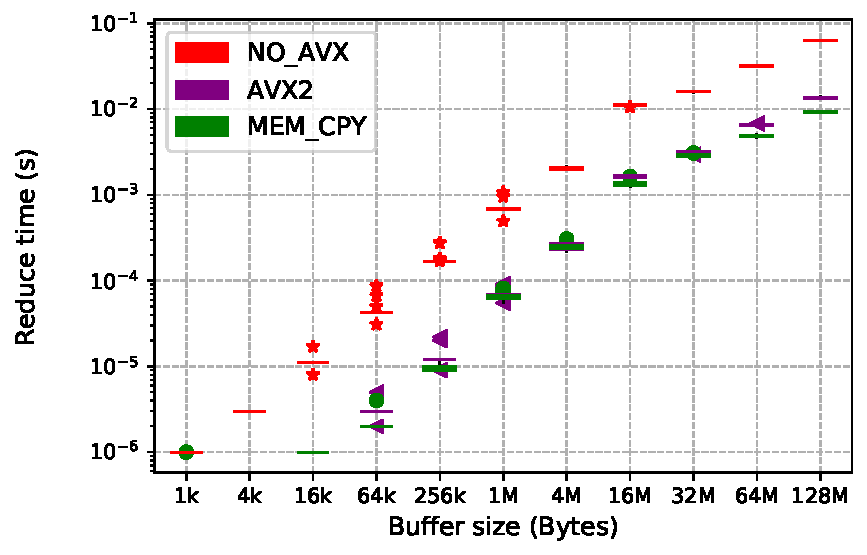
\includegraphics[ width=\linewidth]{amd256_extend_more_sum_u8_1k-128M.pdf}
    \caption{AMD EPYC 7302 16-Core Processor: Comparison of MPI\_SUM with AVX2 reduction enable and disable for MPI\_UINT8\_T together with memcpy}
    \label{fig:amdsum}
\end{figure}

We conducted our benchmark experiments on an EPYC 7302 processor-based cluster,
which is based on the Zen 2 microarchitecture with a base frequency of 3.0 GHz.
It supports AVX and AVX2 instructions.

Figure~\ref{fig:amdsum} show the result for the
\mpifunc{SUM} operation on AMD cluster. We conducted reduction experiments from
different buffer size starts from 1KB to 128MB. We can see that
our AVX2 reduction operations perform five times faster than the default operations
in \ompi for all sizes. When compare with memory copy operations, our optimized operations achieve
almost the same memory bandwidth, which implies we can hide the computation behind memory
operation.

\subsection{Arm-v8 architecture}
\begin{figure}[h]
    \centering
    % trim={<left> <lower> <right> <upper>}
    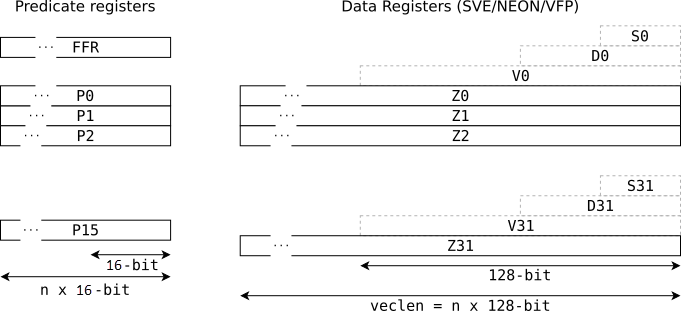
\includegraphics[width=\linewidth]{armsvereg.png}
    \caption{Arm SVE Registers}
    \label{fig:armsvereg}
\end{figure}
Arm introduced Scalable Vector Extension (SVE)~\cite{armSVE2} on the latest Arm-v8 architecture.
As show in figure~\ref{fig:armsvereg}, SVE introduced 16 predicate (P) registers and 32 data (Z) registers,
with the long vector extension, the new architecture
supports vector length starts
from 128 bits up to 2048 bits. It provides a range of different
values that permit vector code to adapt automatically to the
current vector length at runtime with the feature of Vector
Length Agnostic (VLA) programming. Similar to AVX, SVE also has a family of
horizontal reduction instructions
which include integer and floating-point summation, minimum, maximum,
and bit-wise logical reductions.
We implemented our SVE instruction based reduction with Arm
C language extension (ACLE) using intrinsic. As shown in algorithm\ref{fig:svereducealgorithm},
to be noted, ACLE uses agnostic vector length which can be accessed at runtime by
function call of \emph{\textbf{\textit{svcntb() $\mid$ svcnth() $\mid$ svcntw() $\mid$ svcntd()}}}
determines the count the number of 8, 16, 32, 64-bit elements in a vector.
As we mentioned in this paper, \ompi uses a modular architecture,
and we added another SVE reduction module in the operation component. We compile
and install \ompi using Arm HPC compile 20.0 with
flag \emph{\textbf{\textit{-march=armv8-a+sve}}}.

We conducted our performance evaluation experiments of SVE based reduction operation on
the new A64FX processor, which supports vector length of 256 bits and 512 bits.
Figure~\ref{fig:armsum} shows the results of addition operation of \ompi default implementation,
SVE optimized implementation and memory copy operation. We can see that, under all reduction
buffer size, our SVE optimized operation five times faster than element-wise operation.

\begin{algorithm}[ht]
\caption{Arm SVE based reduction algorithm}\label{fig:svereducealgorithm}

\textbf{\textit{types\_per\_step}} \Comment{Number of elements in vector}\\
\textbf{\textit{left\_over}} \Comment{Number of elements waiting for reduction}\\
\textbf{\textit{count}} \Comment{Total number of elements for reduction operation}\\
\textbf{\textit{in\_buf}} \Comment{Input buffer for reduction operation}\\
\textbf{\textit{inout\_buf}} \Comment{Input and output buffer for reduction operation}\\

\begin{algorithmic}[1]
\Procedure{ReductionOp}{ $in\_buf, inout\_buf, count$ }
%\If {( $blocklen$ $\geqslant$ $svcntb$ )}
  \State{\#svcnt*: Count the number of 8,16,32,64-bit elements in a vector}
  \State $types\_per\_step$ = svcntb $\mid$ svcnth $\mid$ svcntw $\mid$ svcntd
  % \EndIf
  \State{\#pragma unroll}
\For { $k \gets types\_per\_step $ to $ count$}
  \State {svld1 from $in\_buf$}
  \State {svld1 from $inout\_buf$}
  \State {sv\#op\_sign\#size\_z}
  \State {svst1 to $inout\_buf$}
  \State {Update left\_over}
\EndFor
\If {($ left\_over$ $\neq$ $0$ )}
%\tcp*{Duff's device}
  \While{( $left\_over$ $\neq$ $0$ )}{
    \State {Set case\_value}
    \State {\textbf{Switch}(case\_value) : \{8 Cases\}}
    \State {Update left\_over}
  \EndWhile
  }
\EndIf
\EndProcedure
\end{algorithmic}
\end{algorithm}

\begin{figure}[h]
    \centering
    % trim={<left> <lower> <right> <upper>}
    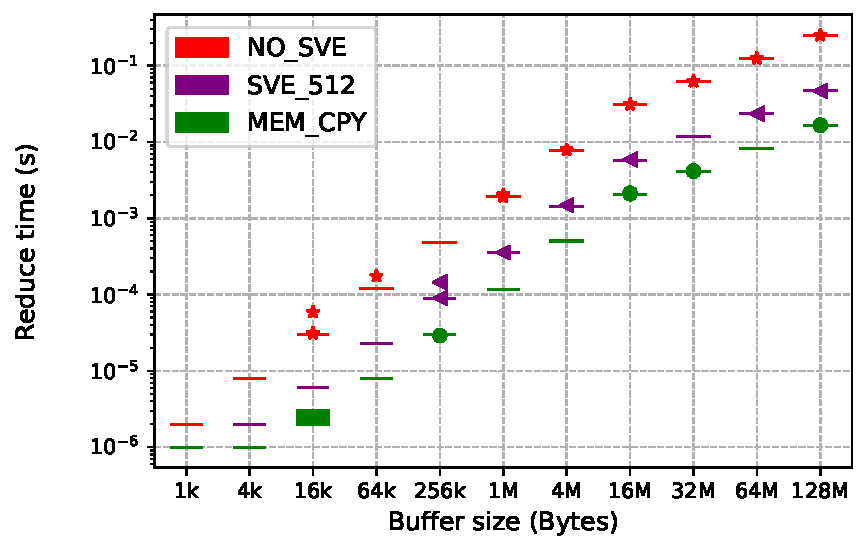
\includegraphics[width=\linewidth]{sve512_extend_more_sum_u8_1k-128M.pdf}
    \caption{Arm A64FX: Comparison of MPI\_SUM with SVE (Vector Length = 512bits) reduction enable and disable for MPI\_UINT8\_T together with memcpy}
    \label{fig:armsum}
\end{figure}

\section{LAMMPS Application Evaluation}\label{sec:hpcapplication}
Large-scale Atomic/Molecular Massively Parallel Simulator (LAMMPS)~\cite{PLIMPTON19951} is a
molecular dynamics simulation tool from Sandia National Laboratories.
It provides different benchmark datasets representing a range of simulation styles
and computational expense for molecular-level interaction forces.
In our experimental analysis, we evaluate the performance of our reduction
operation with LAMMPS granular flow benchmark
using the dataset from chute flow (in.chute.scaled).
The benchmark reports the “Loop Time” as a measure of
time required to simulate a set of interactions.
We run the benchmark with 24 processes (process
grid: 4x2x3) on Intel(R) Xeon(R) Gold 6254 CPU with different
capabilities of AVX support, including single AVX, AVX2 and VX512
and different combination. Different AVXs support combinations can be set using
the modular parameter of \emph{\textbf{\textit{--mca op_avx_support value}}}.

\begin{figure}[h]
    \centering
    % trim={<left> <lower> <right> <upper>}
    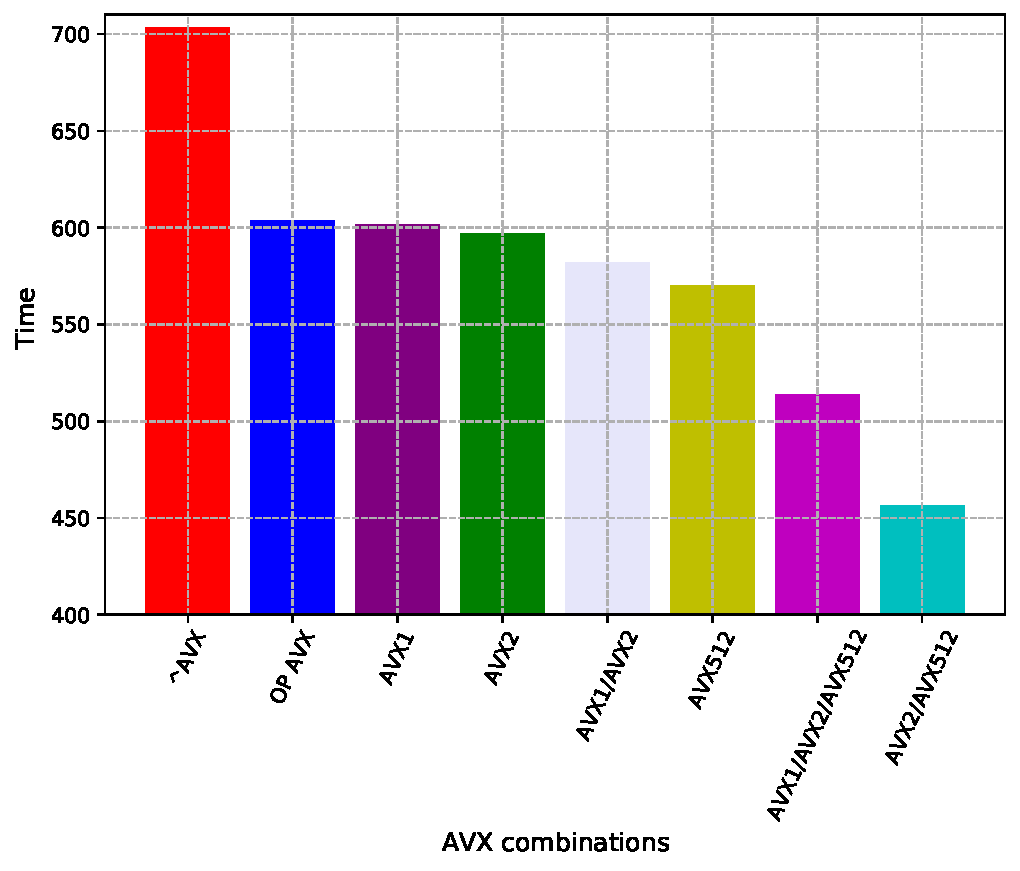
\includegraphics[width=\linewidth]{lammps_avx.pdf}
    \caption{LAMMPS chute: loop time on 24 procs for 100 steps with 259200000 atoms with different AVX capabilities}
    \label{fig:lammpsavx}
\end{figure}

Figure~\ref{fig:lammpsavx} presents the loop time of LAMMPS chute benchmark running
on 24 processes for 100 steps with 259200000 atoms using different AVX capabilities.
Different collective operations are commonly and frequently used in LAMMPS benchmark (eg. \mpifunc{Allreduce}).
We can see, without AVX (option "op $\wedge$ AVX") support in reduction operation as shown in red, the latency of the loop is 700.
With the optimization of using AVX and AVX2, we archive 15\% speedup. After introduced AVX512 our performance
benefit reaches 20\% speedup. With the most optimal combination of AVX2 and AVX512,
we accomplish a speedup of 34\%.

\section{Deep Learning Application Evaluation}\label{sec:application}
Over the past few years, advancements in deep learning have driven
tremendous improvement in image processing, computer vision, speech
recognition, robotics and control, natural language processing, and
many others. One of the significant challenges of deep learning is to
decrease the extremely time-consuming cost of the training process.
%
Designing a deep learning model
requires design space exploration of a large number of hyper-parameters and processing big data.
Thus, accelerating the training process is critical for research and production. Distributed deep learning is one of the essential technologies in reducing training time.
%
The critical aspect to understand in deep learning is that it needs to calculate and update
the gradient to adjust the overall weights.
%
Processes need to prepare and calculate all the gradient data, which is usually very large.
When such data and calculations are too extensive, users need to parallelize these calculations and computations.
%
It indicates the training needs to be executed on distributed computing nodes working
in parallel, and each node works on a subset of the data.
%
When each of these processing units or workers (CPUs, GPUs, TPUs, etc.) is done
calculating the gradient for its subset; they then need to communicate its results
to the rest of the processes involved.

In this section, we investigate and experiment on Horovod~\cite{sergeev2018horovod} - an
open-source component of Michelangelo's deep learning toolkit makes it easier to start and
speed up distributed deep learning projects with TensorFlow.
%
Horovod utilizes \ompi to launch copies of the TensorFlow program. \ompi will transparently set up the distributed infrastructure necessary for processes to communicate with each other. All the user needs to do is to
modify their program to average gradients using an MPI\_Allreduce operation.
%
Conceptually Allreduce has every process to share its data with all other processes and applies a reduction operation.
This operation can be any reduction operation, such as sum, max or min.
In other words, it reduces the target arrays in all processes
to a single array and returns the result array to all processes.
%
Horovod uses a ring-allreduce approach, which is a bandwidth optimal~\cite{allreduce-optimal} algorithm if the tensors are large enough, but does not
work as efficiently for smaller tensors.
Horovod can also use a Tensor Fusion - an algorithm that fuses tensors together
before it calls ring-allreduce. The fusion method allocates a large fusion buffer and executes the
allreduce operation on the fusion buffer.
%
In the ring-allreduce algorithm, each of N nodes communicates with two of its
peers $2 * ($N - 1$)$ times. During this communication, a node sends and receives chunks of the data
buffer. In the first $N - 1$ iterations, received values are added to the values in the node's buffer. In
the second $N - 1$ iterations, after each process receives the data from the previous process, then it
applies the reduction and proceeds to send it again to the next process in the ring.
%
We can see that during the allreduce processing phase, there are $P * ($N - 1$)$ reduction operations
that occurred with big fusion buffer size, which is very computation intensive.
Our AVX-512 optimized reduction operations can significantly improve the performance
of the computation and reduction part of those collective operations.

\begin{figure}[h]
    \centering
    % trim={<left> <lower> <right> <upper>}
    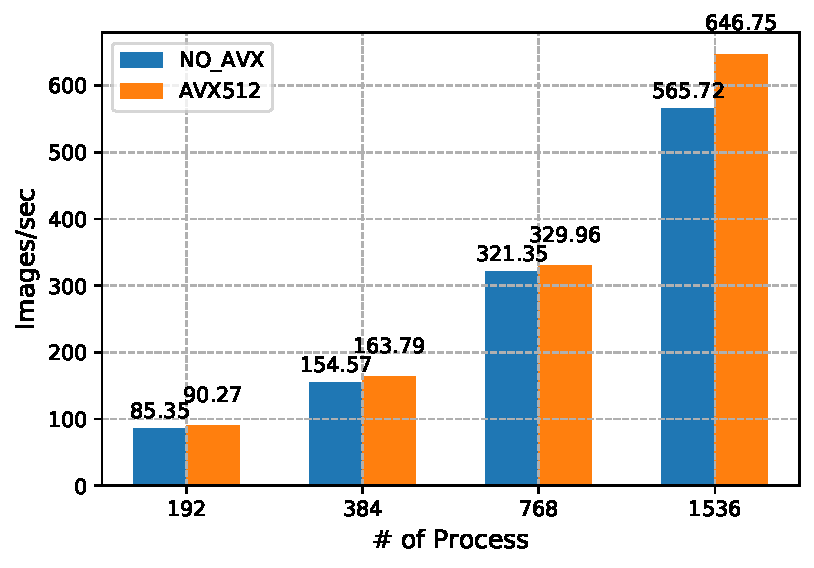
\includegraphics[width=\linewidth]{horovod_tacc.pdf}
    \caption{tf\_cnn\_benchmarks results using Horovod (model: alexnet) on stampede2
    with AVX-512 optimized \ompi and default \ompi}
    \label{fig:horovodtacc}
\end{figure}

We conducted our experiments on Stampede2 with Intel Xeon Platinum 8160 ("Skylake" supports AVX512F) nodes; each node has 48 cores with two sockets. For each node, it has 192GB DDR4 memory. For each core, it has 32KB L1 data cache and 1MB L2. The nodes are connected via Intel Omni-Path network.
We experimented with TensorFlow CNN benchmarks using Horovod with tensorflow-1.13.1.

Figure~\ref{fig:horovodtacc} shows the performance comparison of
our AVX-512 optimized reduction operation and the default reduction operation in \ompi for Horovod (with synthetic datasets and AlexNet model) to train an application called tf\_cnn\_benchmarks~\cite{cnnTensorflow}.
Comparing to default element-wise reduction
implementations, with the increasing number of processes,
our design shows increasing improvements, which start at 5.45\% and
eventually rise to 12.38\% faster than default \ompi on 192 processes and 1536 processes respectively.
We notice that the performance benefit increases with more processes/nodes.
It is because with more MPI processes participated in reduction operation,
the fact that each one of them is simultaneously using our AVX optimized \ompi
operations drives up the overall application performance.

%to do check verbs
\section{Conclusion}\label{sec:conclusion}
In this paper, we pragmatically demonstrated the benefits of Intel
AVX, AVX2, AVX-512 and Arm SVE vector operations in the context of MPI reduction
operations. We assess the performance advantages of different features
introduced by AVX and extended our investigation and analysis to a
fully-fledged implementation of all predefined MPI reduction
operations.
%
We introduced this new reduction operation modules in \ompi using AVXs'
and SVE intrinsic supporting different kinds of \mpi reduce operations for
multiple \mpi types. We demonstrated the efficiency of our vector
reduction operation using a benchmark calling
\mpifunc{Reduce_Local}. Experiments are conducted on an Intel Xeon
Gold cluster, which shows with AVX-512 enabled reduction operations, we
achieve 10X performance benefits.
%
To further validate the performance improvements, experiments are
conducted with different applications: (1) Using LAMMPS benchmark with variety AVX
support show speedup from 14\% to 34\% with different AVX capability combination.
(2) Experiment with a deep learning application
using distributed model Horovod, which calculates and updates the
gradient to adjust the weights using an MPI\_Allreduce.  Our new
reduction strategy achieved a significant speedup across all ranges of
processes, with a 12.38\% improvement with 1536 processes.  Our
analysis and implementation of \ompi optimization provide useful
insights and guidelines on how wide vector operations, in this case,
Intel AVX extensions, can be used in actual high-performance computing
platforms and software to improve the efficiency of parallel runtimes
and applications.
%
% Our AVX512 enabled \ompi provides a better solution for reduction
% operation in general, and in particular on the tested distributed
% neural network training application, the performance is limited by the
% time-consuming reduce calculation, because the number of reductions
% and the data amount are huge.
Our long vector optimized \ompi proves that taking advantage of hardware
capabilities remains of critical interest to software development, and
that even a small improvement in the MPI implementation can have
a significant impact on applications.

\section*{Acknowledgments}
%
This material is based upon work supported by the National Science Foundation under Grant No. (1725692); and the Exascale Computing Project (17-SC-20-SC), a collaborative effort of the
U.S. Department of Energy Office of Science and the National Nuclear Security Administration.
The authors would also like to thank
Texas Advanced Computing Center (TACC). For computer time, this research used
the Stampede2 flagship supercomputer of the Extreme Science and Engineering Discovery Environment (XSEDE) hosted at TACC.

\balance

%
%
%\section*{References}
\bibliographystyle{elsarticle-num}
\bibliography{sample-base}

\end{document}

%%
%% End of file `sample-sigconf.tex'.
\appendix
\end{document}
